\begin{frame}{}
    \begin{textblock*}{55mm}(5mm, 5mm)
        \begin{beamerboxesrounded}{Speckled monster and control}
                By the end of the Middle Ages, smallpox cut down the
            population in centers of Europe and Asia.

                This  ``monster'' represents the first documented
            disease against which a specific control intervention was
            available: the inoculation.
        \end{beamerboxesrounded}
    \end{textblock*}
%
    \begin{textblock*}{115mm}(5mm, 68mm)
        \begin{beamerboxesrounded}{}
            Then Bernoulli naturally sets a question like this: What
            happens if everybody were inoculated? Here, we address the
            question: \textbf{How to  inoculate in an optimal way?}
        \end{beamerboxesrounded}
    \end{textblock*}
%
    \begin{textblock*}{60mm}(70mm, 5mm)
        \begin{bibunit}[apalike]
            \nocite{bradley1971smallpox, Foppa2017}
            \putbib
        \end{bibunit}
    \end{textblock*}
\end{frame}
%
{%
\setbeamertemplate{background canvas}{%
\hskip-2em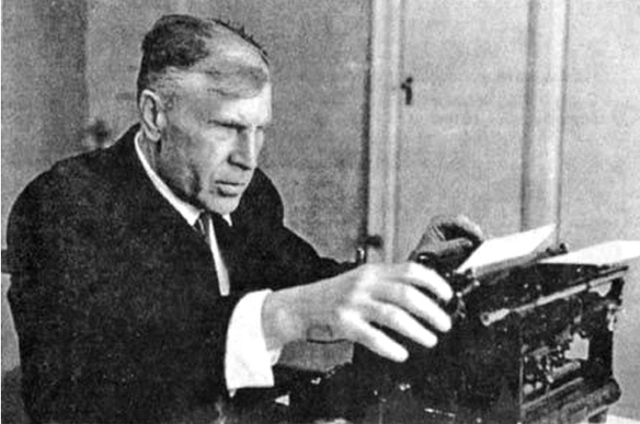
\includegraphics[height=\paperheight]{LevPontriaguin}}
\setbeamercolor{itemize item}{fg=structure.fg!45}
\begin{frame}[plain,t]
    \vfill
    \hfill
    \begin{minipage}{.60\textwidth}
        \usebeamercolor[bg]{normal text}
        \hspace{1em}
        \textbf{\large Lev Semenovich Pontryagin \\
            \hspace*{0.47cm} (1908-1988)}
        \begin{itemize}
        \usebeamercolor[bg]{normal text}
            \item
                Soviet mathematician. He was born in Moscow and lost his
                eyesight due to a primus stove explosion when he was 14.
            \item
                He was able to become one of the greatest
                mathematicians of the 20th century, partially with the help of
                his mother Tatyana Andreevna who read mathematical books and
                papers (notably those of Heinz Hopf, J. H. C. Whitehead, and
                Hassler Whitney) to him.
            \item
                He made major discoveries in a number
                of fields of mathematics, including algebraic topology and
                differential topology.
        \end{itemize}
    \end{minipage}
    \bigskip
\end{frame}
\usebeamercolor[bg]{normal text}
}
%
{%
\setbeamertemplate{background canvas}{%
\hskip-2em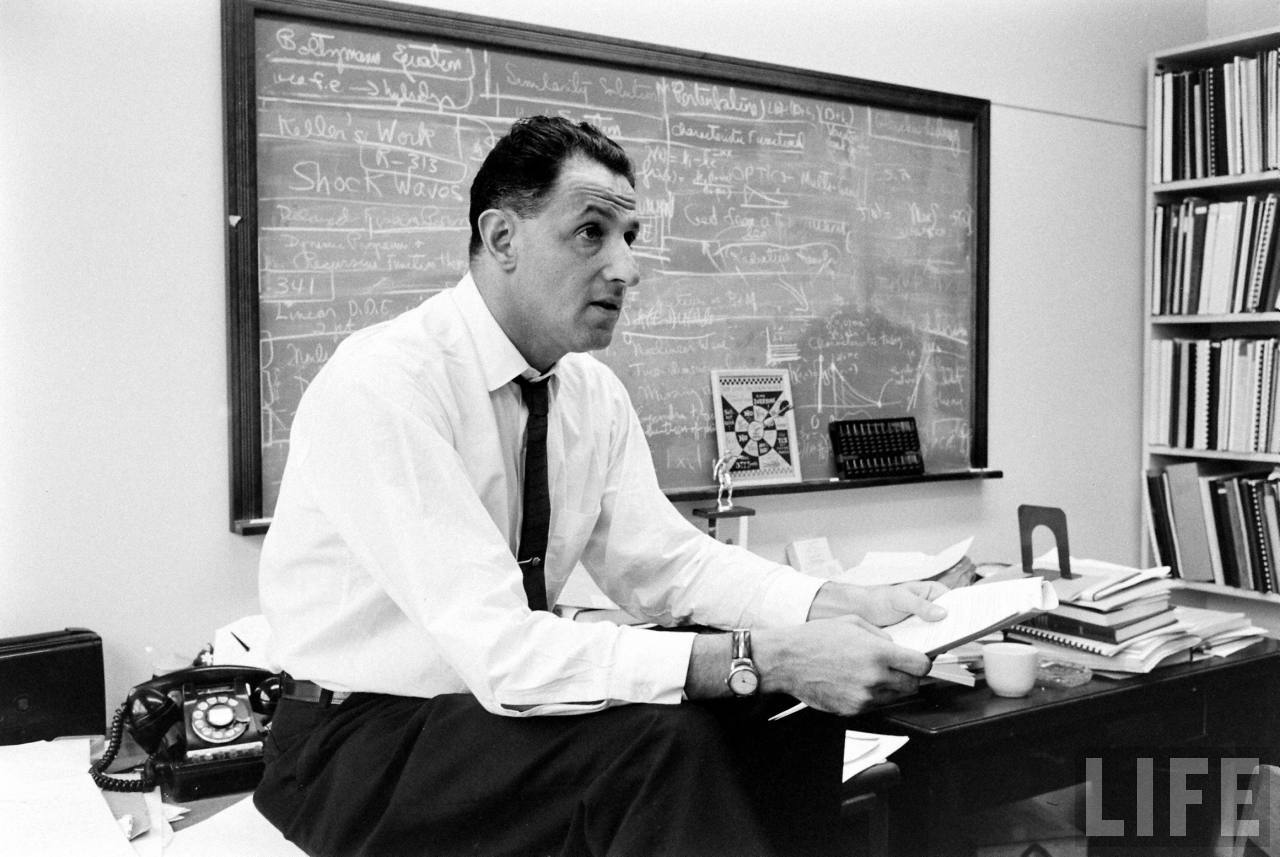
\includegraphics[height=\paperheight]{RichardBellman}}
\setbeamercolor{itemize item}{fg=structure.fg!45}
\begin{frame}

\end{frame}
}

{%
\setbeamertemplate{background canvas}{%
\hskip-2em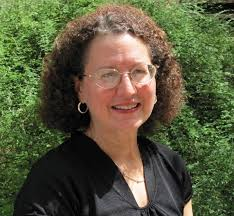
\includegraphics[width=1.2\paperwidth]{SuzanneLenhart}}
\begin{frame}{}
    \only<2->{
    \begin{textblock*}{55mm}(2mm, 5mm)
        \begin{beamerboxesrounded}{Optimal control theory is a way.}
                In the fifties, \textbf{Pontryagin} and
            \textbf{Bellman} propose generalizations of the calculus
            of variations of broader applicability:
            \begin{itemize}
                \item
                    the Maximum Principle
                \item
                    and the method of Dynamic Programming,
            \end{itemize}
            respectively.
        \end{beamerboxesrounded}
    \end{textblock*}
    }
%
    \only<3->{
    \begin{textblock*}{120mm}(5mm, 70mm)
        \begin{beamerboxesrounded}{}
            \begin{bibunit}[apalike]
                \nocite{lenhart2007optimal}
                \putbib
            \end{bibunit}
        \end{beamerboxesrounded}
    \end{textblock*}
    }
\end{frame}
}
